\section{Results}
\label{sec:Results}
\subsection{Current Consumption}
\label{subsec:DigiCurrent}
The current consumption of the digital and analogue circuits recorded during the irradiation of a CBC3 at 23\kGyH is shown in \Cref{fig:DigiCurrent}. 

\begin{figure}[!htbp]
\centering
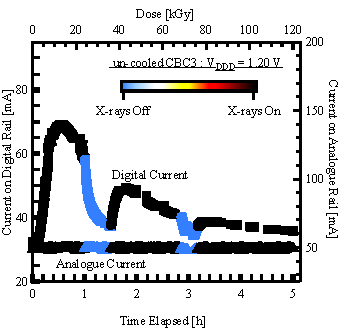
\includegraphics[width=0.8\linewidth]{Figures/DigiCurrent_CBC3_Uncooled.pdf}
\vspace*{-2mm}
\caption{Measured CBC3 digital (left axis) and analogue (right axis) currents during 
exposure to X-rays at the CERN X-ray irradiation facility. The color of the marker indicates the state of the X-ray machine during the measurement. 
%The cooling system was not active during this measurement.
}
\label{fig:DigiCurrent}
\end{figure}
% Needs a way to distinguish analogue from digital on the plot (S.S. too many points for the legend to be very useful... so added a label above each curve instead ) 
% Remove or explain arrows (S.S done!)
As with the previous version of the chip, a radiation-induced leakage current is observed for the CBC3.
%The radiation-induced leakage current observed in the previous version of the chip is still present in the CBC3.
The current consumed begins to increase after a few \kGy of dose and continues to increase up to a dose of approximately $15$\kGy beyond which it decreases exponentially towards the initial value.

% The dose rate and temperature of the CBC3 during the initial irradiation were not representative of those expected in the CMS OT. 
The initial irradiation was performed at a dose rate ${10^{4}}$ times higher than that expected for the 2S modules closest to the interaction point, with chips ${47}$\deg warmer than expected in the Phase-2 OT. Determining the magnitude of the current increase under realistic HL-LHC operating conditions therefore requires an understanding of the effect of temperature and dose rate on the radiation induced leakage current. This motivated the undertaking of a series of measurements at different temperatures and dose rates summarized in \Cref{fig:DigiCurrentSummary}.
%\cite{BragaThesis}
\begin{figure}[!htbp]
\centering
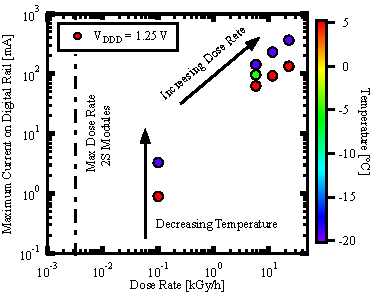
\includegraphics[width=0.8\linewidth]{Figures/DigiCurrent_CBC3_Summary_v2.pdf}
\vspace*{-5mm}
\caption{The (maximum) measured current consumption on the CBC3 digital rail as a function of dose rate. The color of the markers indicates the temperature at which the irradiation took place. All measurements used a bias voltage of $1.25$\,\volt.}
\label{fig:DigiCurrentSummary}
\end{figure}

The measured radiation induced increase in current rises for decreasing temperatures and increasing dose rates. The temperature of the CBCs when deployed in the Phase-2 OT will range from ${-17}$\deg to ${-9}$\deg; and the expected dose rate, indicated by a dashed line in \Cref{fig:DigiCurrentSummary}, is approximately $2$\% of the lowest dose rate reached in the X-ray irradiations. 

\subsection{Analogue Front-End Performance}
To verify robustness of the CBC3 analogue front-end against damage from ionizing radiation all parameters critical to its operation were monitored throughout. This included checking the behavior of  analogue bias registers, verification of  on-chip pipeline by measuring the response to the internal test pulse, and continuous monitoring of the pedestal and the noise.

% The CBC3 derives all analogue biases in the front end circuits using an on-chip bias generation circuit referenced by a radiation tolerant, PMOS transistor based, voltage reference bandgap. 
The two most important analogue biases are: the output of the band-gap reference ($V_{BG}$) circuit and the comparator threshold voltage ($V_{cth}$). $V_{BG}$ is the reference for all on-chip analogue biases, and $V_{cth}$ determines the global comparator threshold (shown in \Cref{fig:Architecture_AnalogueFE}). The resolution of $V_{th}$, provided by a 10 bit digital to analogue converter (DAC) with reference voltages provided by the analogue supply rail ($V_{DDA}$) and the on-chip ground (GND), is given by
\begin{equation}
V_{cth}\,\,[\frac{\mbox{\mV}}{\mbox{DAC units}}]=\frac{V_{DDA} - GND}{1024}=\frac{2V_{BG}-GND}{1024},
\label{eq:Vcth}
\end{equation}
where $V_{DDA}$ is twice $V_{BG}$. 
\begin{figure}[htbp]
\centering
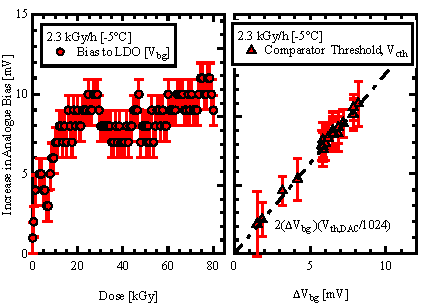
\includegraphics[width=0.9\linewidth]{Figures/Vbg_Irrad_v2.pdf}
\vspace*{-2mm}
\caption{$V_{BG}$ and $V_{cth}$ during irradiation; the comparator threshold corresponds to the output of the bias DAC at the nominal threshold setting of $\approx$580 DAC units.}
\label{fig:Vbg}
\end{figure}
%S.S. combined what was previously figures 6 and 7 into one plot - hopefully its not too squished in.

The evolution of the band-gap reference voltage during irradiation, and the corresponding change in $V_{cth}$, for a chip irradiated at $2.3$\kGyH and a temperature of -5\deg is shown in \Cref{fig:Vbg}. The measured $10$\mV\! increase (${O(2\%)}$) in the band-gap reference voltage of the chip is within the expected range (${\pm 12}$\mV\!) for the circuit used in the CBC3 \cite{Bandgap}; and the increase in threshold voltage is as expected from \Cref{eq:Vcth}. 

%I don't think I have enough space to show this 
% And then what about the noise? Complicated by the fact the cooling started before the start of the irradiation ...
% \begin{figure}[htbp]
% \centering
% 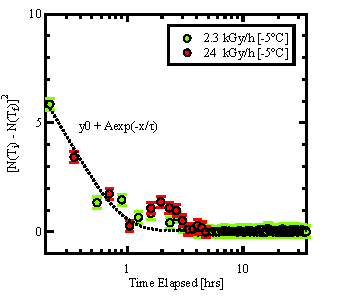
\includegraphics[width=0.8\linewidth]{Figures/Noise2_IncreaseIrrad.pdf}
% \caption{The size of reconstructed clusters in strips (635 $\mu$m
% strip pitch) for both readout coordinates of the central detector.}
% \label{fig:Noise2}
% \end{figure}
% Seems to be correlated with the increase in digital current. 
% \begin{figure}[htbp]
% \centering
% 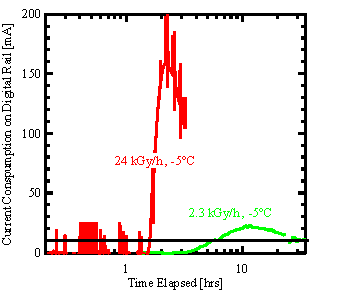
\includegraphics[width=0.8\linewidth]{Figures/Current_IncreaseIrrad.pdf}
% \caption{The size of reconstructed clusters in strips (635 $\mu$m
% strip pitch) for both readout coordinates of the central detector.}
% \label{fig:CurrentIncrease}
% \end{figure}

\begin{figure}[!htbp]
\centering
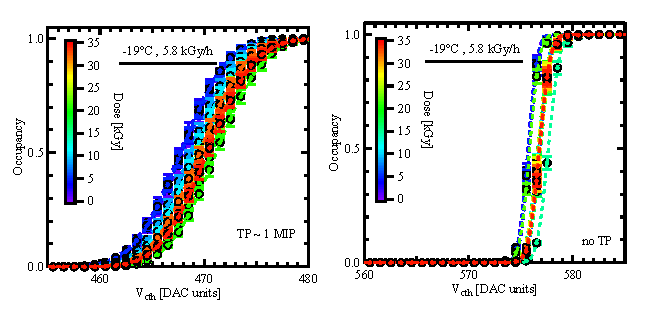
\includegraphics[width=1.1\linewidth]{Figures/Scurves_Chip4.pdf}
%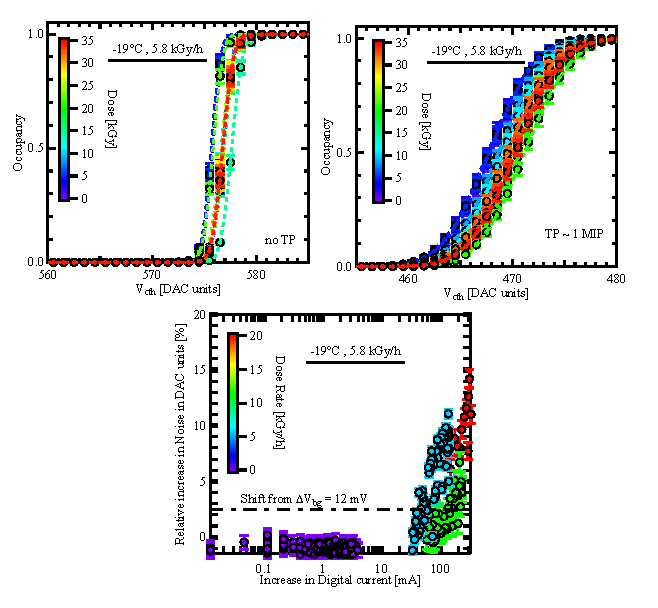
\includegraphics[width=0.99\linewidth]{Figures/test.pdf}
%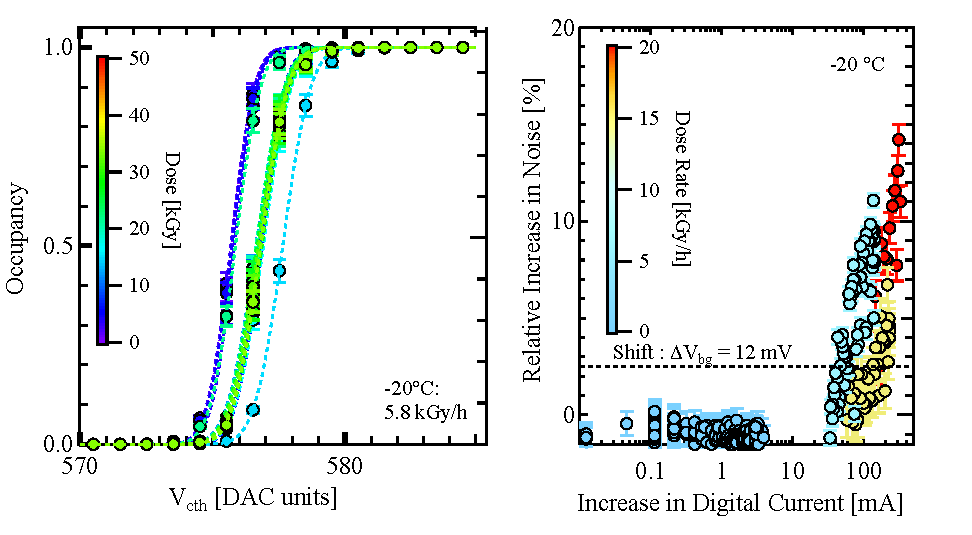
\includegraphics[width=1.1\linewidth]{Figures/NoiseIncrease_Summary_Chip4.pdf}
\vspace*{-10mm}
\caption{S-curves measured during the irradiation period: (left) using the on-chip test pulse to inject charge equivalent to 1 MIP, and (right) with no charge injected.The color of the markers indicates the dose received at the time of measurement, and the dashed lines the result of the fit using \Cref{eq:scurve}.}
\label{fig:Scurves}
\end{figure}

The noise and pedestal in a binary system such as the CBC3 must be inferred from an S-curve which shows the fraction of events in which a hit is detected as a function of the comparator threshold $V_{cth}$. Examples of S-curves collected during an irradiation are shown in \Cref{fig:Scurves}. Fitting the S-curve with a sigmoid of the form :
\begin{equation}
f(x, \mu, \sigma) =\frac{1}{2}[1 + \erf(\frac{x-\mu}{\sqrt{2}\sigma}) ],
\label{eq:scurve}
\end{equation}
returns the  pedestal (\textmu) and noise ($\sigma$). S-curves were also used to test the response of the CBC3 to the internal test pulse, by using the on-chip test pulse to inject charge into all 254 input channels on the CBC3. 
%missing \cite{BragaThesis}
%can be extracted directly from the S-curves by fitting them with a sigmoid of the form where \textmu and $\sigma$ correspond to the pedestal the noise respectively.  
As \Cref{fig:Scurves} shows, the CBC3 remains responsive to the test pulse in the presence of a large leakage current (${\approx 200}$\mA). This indicates that enclosed pipeline transistors in the CBC3 mitigated effects observed in the previous version. The noise and pedestals measured for different dose rates are shown in \Cref{fig:noisePede}. It shows that the increase in noise observed during irradiation at high dose rate is correlated with the radiation induced leakage current; no change in noise is observed as long as the increase in current remains below ${10}$\mA.


\begin{figure}[!htbp]
\centering
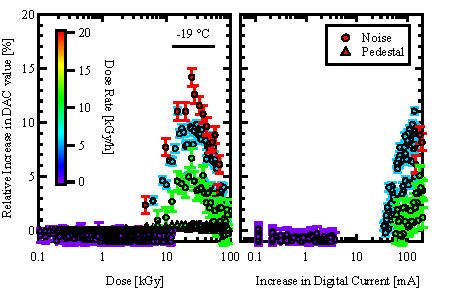
\includegraphics[width=0.9\linewidth]{Figures/NoisePede_Summary.pdf}
%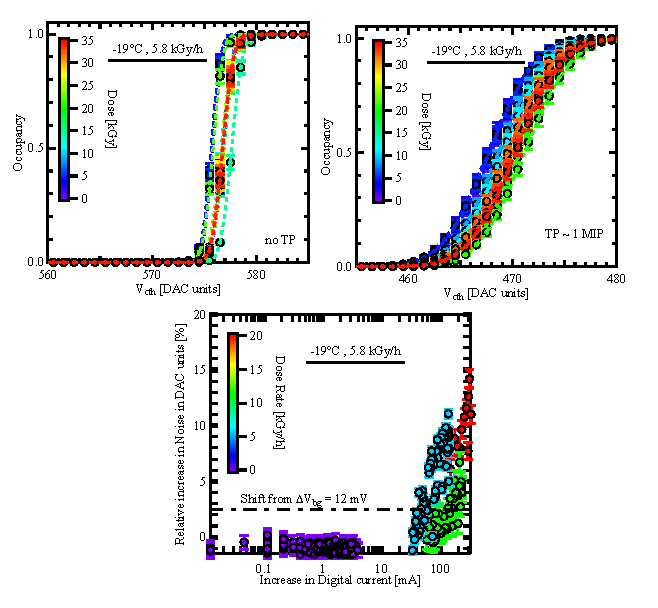
\includegraphics[width=0.99\linewidth]{Figures/test.pdf}
%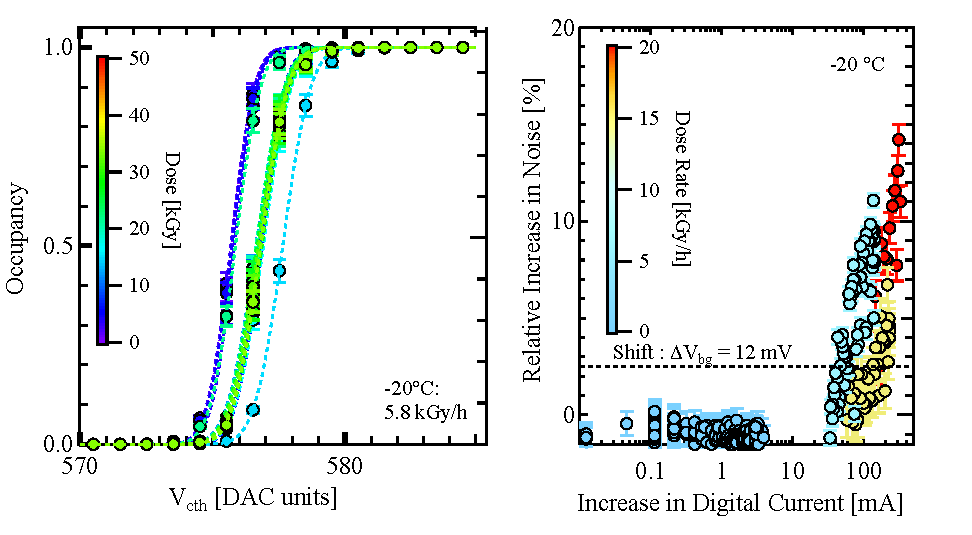
\includegraphics[width=1.1\linewidth]{Figures/NoiseIncrease_Summary_Chip4.pdf}
\vspace*{-2mm}
\caption{Noise and pedestal as a function of dose(left) , and correlation between noise and increase in digital current (right).The color of the markers indicates the dose rate at which the irradiation took place.}
\label{fig:noisePede}
\end{figure}

%Summarize performance ... and motivate radiation damage model 


%$-19$\deg can be used to place an upper limit on the maximum current expected in the CBCs in the Phase-2 OT conditions